%%%%%%%%%%%%%%%%%%%%%%%%%%%%%%%%%%%%%%%%%%%%%%%
% CL provided template
%%%%%%%%%%%%%%%%%%%%%%%%%%%%%%%%%%%%%%%%%%%%%%%

\documentclass[12pt,a4paper,oneside,openright]{report}

% makes subsubsections appear in the toc
\setcounter{secnumdepth}{3}
\setcounter{tocdepth}{3}

% turns references into hyperlinks
\usepackage[pdfborder={0 0 0}]{hyperref}
\newcommand{\URL}[1]{\href{https://#1}{\textcolor{cyan}{\texttt{#1}}}}

\usepackage{tablefootnote}

% adjusts page layout
\usepackage[margin=25mm]{geometry}

% allows inclusion of PDF, PNG and JPG images
\usepackage{graphicx}
\graphicspath{ {figs/} }

\usepackage{verbatim}

% try to avoid widows and orphans
\raggedbottom
\sloppy
\clubpenalty1000%
\widowpenalty1000%

% adjust line spacing to make more readable
\renewcommand{\baselinestretch}{1.1}

% add colour to TODOs
\usepackage{xcolor}

%%%%%%%%%%%%%%%%%%%%%%%%%%%%%%%%%%%%%%%%%%%%%%%
% Maths
%%%%%%%%%%%%%%%%%%%%%%%%%%%%%%%%%%%%%%%%%%%%%%%

\usepackage{amsmath}        % American Mathematical Society
\usepackage{amssymb}        % Maths symbols
\usepackage{amsthm}         % Theorems
\usepackage{mathpartir}    % Proofs and inference rules

%%%%%%%%%%%%%%%%%%%%%%%%%%%%%%%%%%%%%%%%%%%%%%%
% Floats
%%%%%%%%%%%%%%%%%%%%%%%%%%%%%%%%%%%%%%%%%%%%%%%

\usepackage{float}
\usepackage[labelfont=bf,margin=10pt]{caption}
\usepackage{subcaption}
\newcommand{\mycaption}[2]{\caption[#1]{#1 #2}}

\floatstyle{plain}
\restylefloat{figure}
\restylefloat{table}

%%%%%%%%%%%%%%%%%%%%%%%%%%%%%%%%%%%%%%%%%%%%%%% 
% Figures
%%%%%%%%%%%%%%%%%%%%%%%%%%%%%%%%%%%%%%%%%%%%%%%

\usepackage{tikz}
% Shamelessly stolen to draw VBox diagrams
\usepackage{threads}

%%%%%%%%%%%%%%%%%%%%%%%%%%%%%%%%%%%%%%%%%%%%%%%
% Tables
%%%%%%%%%%%%%%%%%%%%%%%%%%%%%%%%%%%%%%%%%%%%%%%

\usepackage{array}
% control width and vertically align text in table cells
\newcolumntype{L}[1]{>{\raggedright\let\newline\\\arraybackslash\hspace{0pt}}p{#1}}
\newcolumntype{C}[1]{>{\centering\let\newline\\\arraybackslash\hspace{0pt}}p{#1}}
\newcolumntype{R}[1]{>{\raggedleft\let\newline\\\arraybackslash\hspace{0pt}}p{#1}}

%%%%%%%%%%%%%%%%%%%%%%%%%%%%%%%%%%%%%%%%%%%%%%%
% Listings
%%%%%%%%%%%%%%%%%%%%%%%%%%%%%%%%%%%%%%%%%%%%%%%

\usepackage{fancyvrb}

\floatstyle{boxed}
%\floatstyle{ruled}
\newfloat{Listing}{tbp}{lol}[chapter]

\DefineVerbatimEnvironment{JavaCode}{Verbatim}
{fontfamily=courier,baselinestretch=1,gobble=4}

\DefineVerbatimEnvironment{GoCode}{Verbatim}
{fontfamily=courier,baselinestretch=1,gobble=4}

\usepackage{listings}
\usepackage{color}
\usepackage{mathtools}

\definecolor{dkgreen}{rgb}{0,0.4,0}
\definecolor{gray}{rgb}{0.5,0.5,0.5}
\definecolor{mauve}{rgb}{0.58,0,0.82}

\lstset{
  language=Java,
  aboveskip=0mm,
  belowskip=0mm,
  showstringspaces=false,
  %columns=flexible,
  basicstyle={\small\ttfamily},
  numbers=left,
  keywordstyle=\bfseries,
  commentstyle=\color{dkgreen},
  stringstyle=\color{mauve},
  breaklines=true,
  breakatwhitespace=true,
  tabsize=4
}


%%%%%%%%%%%%%%%%%%%%%%%%%%%%%%%%%%%%%%%%%%%%%%%
% Semantic and convenience macros
%%%%%%%%%%%%%%%%%%%%%%%%%%%%%%%%%%%%%%%%%%%%%%%

\newcommand{\TOBEDONE}{{\LARGE To be done...}}
\newcommand{\todo}[1]{\textcolor{red}{TODO: #1}}
\newcommand{\note}[1]{\textcolor{blue}{NOTE: #1}}

\newcommand{\javaLiteral}[1]{\texttt{#1}}
\newcommand{\javaCode}[1]{\texttt{#1}}
\newcommand{\javaClass}[1]{\texttt{#1}}
\newcommand{\javaSlot}[1]{\texttt{#1}}
\newcommand{\javaVariable}[1]{\texttt{#1}}
\newcommand{\javaKeyword}[1]{\texttt{#1}}
\newcommand{\javaMethod}[1]{\texttt{#1}}
\newcommand{\javaException}[1]{\texttt{#1}}
\newcommand{\javaAnnotation}[1]{\texttt{#1}}

\newcommand{\goCode}[1]{\texttt{#1}}
\newcommand{\goType}[1]{\texttt{#1}}
\newcommand{\goValue}[1]{\texttt{#1}}
\newcommand{\goVariable}[1]{\texttt{#1}}
\newcommand{\goKeyword}[1]{\texttt{#1}}
\newcommand{\goFunc}[1]{\texttt{#1}}

\newcommand{\keyTerm}[1]{\textbf{#1}}

\newcommand{\codeemph}[1]{\textbf{#1}}

%%%%%%%%%%%%%%%%%%%%%%%%%%%%%%%%%%%%%%%%%%%%%%%
% Info about dissertation
%%%%%%%%%%%%%%%%%%%%%%%%%%%%%%%%%%%%%%%%%%%%%%%

\newcommand{\disstitle}{Software Transactional Memory implementation
  and benchmarking in Go}
\newcommand{\college}{Churchill College}
\newcommand{\studentname}{Rui Cachopo}
\newcommand{\candidatenumber}{2399F} %checked Moodle on 25/04/2020
\newcommand{\studentemail}{rmc82@cam.ac.uk}
\newcommand{\wordcount}{0000}
\newcommand{\loc}{0000}
\newcommand{\originator}{\candidatenumber}
\newcommand{\supervisor}{Tim Harris}

%%%%%%%%%%%%%%%%%%%%%%%%%%%%%%%%%%%%%%%%%%%%%%%
% Start of document
%%%%%%%%%%%%%%%%%%%%%%%%%%%%%%%%%%%%%%%%%%%%%%%

\begin{document}

\bibliographystyle{apalike}

\pagestyle{empty}

%%%%%%%%%%%%%%%%%%%%%%%%%%%%%%%%%%%%%%%%%%%%%%%
% Cover page
%%%%%%%%%%%%%%%%%%%%%%%%%%%%%%%%%%%%%%%%%%%%%%%

\rightline{\LARGE \textbf{\studentname}}

\vspace*{60mm}
\begin{center}
  \Huge
  \textbf{\disstitle} \\[5mm]
  Computer Science Tripos -- Part II \\[5mm]
  \college \\[5mm]
  \today
\end{center}

\newpage

\section*{Declaration}

I, \studentname\ of \college, being a candidate for Part II of the
Computer Science Tripos, hereby declare that this dissertation and the
work described in it are my own work, unaided except as may be
specified below, and that the dissertation does not contain material
that has already been used to any substantial extent for a comparable
purpose.

I, \studentname\ of \college, am content for my dissertation to be
made available to the students and staff of the University.

\bigskip \leftline{Signed: }

\medskip \leftline{Date: \today}


\chapter*{\vspace{-1.2in} Proforma \vspace{-0.3in}}

\thispagestyle{empty}

\vspace{-0.2in}

\begin{table}[h]
  \begin{tabular}{L{0.3\linewidth} L{0.7\linewidth}}
    \textbf{Candidate number:} & \candidatenumber                      \\
    \textbf{Project Title:}           & \disstitle \\
    \textbf{Examination:}        & Computer Science Tripos -- Part II, July 2020  \\
    \textbf{Word Count:}         & \wordcount\tablefootnote{According to
                                   the command provided with the
                                   dissertation template: \\ \indent \indent
    \indent \texttt{detex
    diss.tex | tr -cd '0-9A-Za-z
    \char`\\ n' | wc -w}} \\
    \textbf{Lines of code:} & \loc\tablefootnote{Calculated using
                              Github's contributions feature.} \\
    \textbf{Project Originator:} & \originator \\
    \textbf{Supervisor:} & \supervisor \\
  \end{tabular}
\end{table}

\vspace{-0.4in}

\section*{Original Aims of the Project}

The core goals of the project were to implement a Software
Transactional Memory and to make a meaningful evaluation of the system
produced. This evaluation involves both quantitative benchmark results
and qualitative results related to the usability of the system. The
technical deliverables are implementations of the STM and the
benchmark produced --- as there is no existing realistic benchmark in
the language chosen for this project. The qualitative results of the
evaluation can be found in the evaluation chapter of this
dissertation.

\vspace{-0.1in}

\section*{Work Completed}

All the success criteria of the project have been met. I implemented
the Go Versioned Software Transactional Memory and demonstrated its
correctness and performance by producing an implementation of the
STMBench7 benchmark and accompanying tests. Due to the difficulties
described in the section below I had much less time than I had hoped
to work on extension tasks.

The completion of this work required substantial research into
Transactional Memory and Go's concurrency primitives and memory
model. Implementation of an application as large as the STMBench7
benchmark also required knowledge and use of software engineering
patterns and practices.

\vspace{-0.1in}

\section*{Special Difficulties}

In November 2019 I had a climbing accident that resulted in a
dislocated elbow. This halted project work, and in fact all academic
work, for a few weeks until I was able to use a keyboard again.

Starting in March 2020, the COVID-19 pandemic forced me, and indeed
the vast majority of students, to work from home for the rest of the
academic year. This meant that the last month of work on the project
and this dissertation were completed in an environment much less
productive than expected.

\newpage

\pagestyle{plain} \pagenumbering{roman}

\tableofcontents

\listoffigures{}

\listoftables{}

\listof{Listing}{List of Listings}

\newpage

\section*{Acknowledgements}


%%%%%%%%%%%%%%%%%%%%%%%%%%%%%%%%%%%%%%%%%%%%%%%
% #Content
%%%%%%%%%%%%%%%%%%%%%%%%%%%%%%%%%%%%%%%%%%%%%%%

\pagestyle{headings}

%%%%%%%%%%%%%%%%%%%%%%%%%%%%%%%%%%%%%%%%%%%%%%%
% Intro
%%%%%%%%%%%%%%%%%%%%%%%%%%%%%%%%%%%%%%%%%%%%%%%

\chapter{Introduction}

\pagenumbering{arabic}

This dissertation describes the implementation and benchmarking of a
Software Transactional Memory (STM) in Go, a programming language that
emerged just as research on STMs dwindled. In this chapter I aim to
give a brief historical background of STMs and explain the choices I
made when proposing the project. In particular, I explain the choice
of STM algorithm, programming language and benchmark to use.

\section{Motivation and previous work}
\label{sec:motivation}

To have some context on the motivations behind STMs, it makes most
sense to first remember the historical trends in processor
design. From there, we can see how modern hardware limitations caused
a revolution in software and the problems that this caused to
programmers. Finally, we can see how STM tackles these problems.

\subsection{The problem}
\label{sec:problem}

In the last few decades, and especially in the period of 1986--2003,
single-core processor performance grew exponentially at such a rate
that hardware became obsolete within one or two years. This was mostly
thanks to two ``laws'' of processor design: Moore's
law~\cite{MooreLaw} and Dennard scaling~\cite{DennardScaling}. Moore's
law is the observation that, due to the production of smaller
transistors, the number of transistors in a processor doubles every
two years. Although the prediction in the 1965 paper was a doubling in
transistor count every year, this was revised in 1975 to a doubling
every two years. Dennard scaling states that as transistors get
smaller and consume less power, their power density stays constant, so
the power consumption of the whole processor remains constant.

The combination of these laws impacts processor performance in three
main ways:

\begin{itemize}
\item Smaller transistors can switch faster, meaning that the clock
  frequency of the processor can be increased.
  
\item The higher transistor budget allows for more complex hardware
  design. One way this was exploited was the use of pipelining, which
  reduces the critical path inside processor and allows the clock
  frequency of the processor to increase.
  
\item More complex hardware design was also used to build
  out-of-order, superscalar processors. These processors could exploit
  Instruction Level Parallelism (ILP)~\cite[Chapter~3]{CompArchBook}
  latent in most programs.
\end{itemize}
This processor performance ``free lunch''~\cite{FreeLunchIsOver} ended
in the early 2000s, when Dennard scaling ceased to hold and the
low-hanging fruit of processor design had been harvested:

\begin{itemize}
\item In post-Dennard scaling, power consumption becomes a limiting
  factor in the complexity of a single core and on the clock frequency
  of the processor.
  
\item The performance penalties caused by processor stalls, such as
  cache misses and mispredicted branches, increases with the length of
  the processor pipeline. This means deeper pipelines yield
  diminishing returns.
  
\item The amount of ILP latent in most programs is limited. This means
  that increasingly complex superscalar hardware will also yield
  diminishing returns.
\end{itemize}
As the limits of single-core performance and latent ILP were reached,
processor designers shifted their focus to multicore processors, which
are capable of exploiting Thread Level Parallelism
(TLP)~\cite[Chapter~5]{CompArchBook}. As opposed to ILP, which can be
automatically exploited by the processor in most applications, TLP
usually requires the program to be written using multiple
threads. This means that the burden is now on programmers to write
concurrent applications if they want to reap the benefits of
increasing processor performance. Enter the software revolution
towards concurrent programming.

\subsection{Possible solutions}
\label{sec:possible-solutions}

\paragraph{Locking.} The model most commonly used in concurrent
programs consists of multiple threads, which communicate through
access to shared memory. Low level primitives such as locks are used
to provide condition synchronisation and mutual exclusion when
accessing shared resources. This model is sufficient for simple
programs, but it does not scale to large applications. Problems such
as deadlock and priority inversion are hard to detect and debug in
large programs. The lack of a semantic link between a mutex lock and
the resource it protects leads to what Herlihy and Shavit call
``synchronisation by convention''~\cite[Chapter
18]{ArtMultiprocessorProgramming}.

\begin{Listing}[hbtp]
\begin{lstlisting}
/* When a locked buffer is visible to the I/O layer BH_Launder
 * is set. This means before unlocking we must clear BH_Launder,
 * mb() on alpha and then clear BH_Lock, so no reader can see
 * BH_Launder set on an unlocked buffer and then risk to
 * deadlock.
 * /
\end{lstlisting}

  \mycaption{Synchronisation by convention.}{This Linux kernel comment
    demonstrates how real-world concurrent systems rapidly become
    complex.}
  \label{lst:syncConv}
\end{Listing}


\paragraph{Monitors and condition variables.} Several approaches have
been suggested as solutions to the problems present when using locks
and shared memory. The most basic of these is the use of slightly
higher level primitives, such as monitors and condition
variables. Java is a good example of this: the JVM associates one
monitor and one condition variable with each object. A
\javaKeyword{synchronized} code block runs inside a monitor, which can
be used to provide mutual exclusion. The condition variables can be
used for condition synchronisation using the \javaMethod{wait},
\javaMethod{notify} and \javaMethod{notifyAll} methods.

\paragraph{Message passing.} Moving away from threads and shared
memory, other concurrency models have been created. The most
widespread involve message passing between strongly isolated processes
--- so called because, unlike threads, they do not share
memory. Hoare's Communicating Sequential Processes~\cite{CSP} and
Milner's Calculus of Communicating Systems~\cite{CCS} are two formal
models that use this idea. These models are mostly employed by
functional programming languages such as Erlang, which allow no shared
memory and in which all data is immutable. Concurrent programs in
these languages can be simpler to write and debug, but often do not
perform as well as programs written in more ``traditional'' languages
such as Java and C\texttt{++}.

\paragraph{Transactional memory.} Yet another approach, and the focus
of this dissertation, is Transactional Memory (TM)~\cite{TMBook}. When
using transactional memory, a programmer organises their code into
transactions, similar to the transactions in the transactional model
of databases. It is then up to the underlying TM implementation to
provide atomicity and isolation of the transactions executed. That is,
the memory operations of each transaction executed appear to occur
atomically, and no transaction can see the results of a partial
execution of any other transaction.

\subsection{Transactional memory}
\label{sec:transactional-memory}

Transactional memories provide a very simple interface to programmers:
to write a correct concurrent program, place all parallel code that
accesses shared data inside transactions, and let the underlying TM
ensure the program is correctly synchronised. Transactional memories
also provide composability, meaning it is simple to compose existing
transactions to achieve more complex behaviour. As an example,
consider that we want to dequeue an element from a concurrent queue
$Q_1$ and enqueue it in concurrent queue $Q_2$, but without any other
thread observing that the element is in neither or both queues at the
same time. Attempting to solve this problem with locks would be fairly
complex, involving either additional locks or exposing the internal
locking logic of the concurrent queues. In a TM model, however, the
solution is trivial: simply execute both operations in the same
transaction.. This is discussed in more depth in Section
\ref{sec:prep:techn-requ}.

Transactional memories can be implemented in hardware or
software. Hardware Transactional Memories (HTM) \todo{citation} are
usually implemented on top of the cache coherence protocol of a
processor, and are offered as an Instruction Set Architecture (ISA)
extension. Because they operate at such a low level, HTMs are often
very efficient, but the size of transactions is limited by the size of
cache available and the implementation cost is extremely
high. Software Transactional Memories (STM)~\cite{STM} are much more
flexible, but implementing them efficiently can be a
challenge. Efficiency concerns with regards to STMs are so great that
they have been called a ``research toy''~\cite{Toy}.

\section{Golang}
\label{sec:intro:golang}

In this project I aim to implement an STM and evaluate its
performance. I have chosen to do this in Go\footnote{\URL{golang.org}}
because it is a language that emerged after the wave of research on
STMs in the early 2000s, and so there is no exploration of how the
language's features can be exploited to increase the applicability of
STM approaches. Additionally, Go is designed with concurrency as a
primary focus. In fact, one of the primary uses of Go has been to
build server applications, and there is a growing environment of tools
and libraries to support this. Examples are Docker and Kubernetes
implementations, the etcd key-value store
system\footnote{\URL{etcd.io}}, the Elasticsearch-Logstash-Kibana
stack for logging\footnote{\URL{elastic.co/what-is/elk-stack}} and
Prometheus for metric tracking\footnote{\URL{prometheus.io}}. One of
my goals when choosing to use Go for this project was to eventually
contribute to this environment, and make it easy for software
engineers to build server applications using STM.

\section{The STM chosen}
\label{sec:stm-chosen}

Although there has been substantial research on the topic of
transactional memory, and many STMs have been implemented, there are
few applications that actually use them. From a software engineering
perspective, there are many possible reasons for this, such as
adoption costs and little to no support of commonly used libraries. As
one of my goals in choosing my project was to one day develop an STM
that could be adopted in industry, it made sense to base my project on
an existing STM with a real-world application. Such an STM is the Java
Versioned Software Transactional Memory
(JVSTM)\footnote{\URL{web.ist.utl.pt/joao.cachopo/jvstm/}}, which has
been used in the FenixEDU
project~\cite{carvalho2008versioned}. Because my STM uses the same
version box--based algorithm~\cite{VBox} but is implemented in Go
instead of Java, I have decided to name it Go Versioned Software
Transactional Memory (GVSTM).

\section{Evaluation and benchmarking}
\label{sec:eval-benchm}

Performance is a crucial factor in the evaluation of STMs. Although it
has been shown that STMs can largely outperform sequential code in
multicore computers~\cite{MoreThanToy}, it falls to each STM
implementation to show that it is sufficiently efficient to be
adopted. With that goal in mind, it is important for the success of
this project to demonstrate how the STM implemented performs when
compared to alternatives, even if it does not outperform them.

With that in mind, I have chosen to include in the evaluation of my
STM the results of the STMBench7 benchmark, which can be regarded as a
stress test of STMs~\cite{STMBench7}. STMBench7 aims to be a realistic
benchmark, meaning that instead of performing a long series of simple
transactions, such as reading and writing a handful of variables, it
performs elaborate operations on complex data structures. A
description of the benchmark and its data structures and operations
can be found in Section \ref{sec:impl:stmbench7}.

As of the start of this project, there is no Go implementation of
STMBench7. This means that a considerable part of the work to be
completed, both in terms of lines of code written and time investment,
will consist of adapting the existing Java version to be implemented
in Go. Because of the complexity and size of the benchmark, my
proposal is to implement a subset of the original 45
operations. Completing the implementation of the benchmark is an
extension goal of the project.

%%%%%%%%%%%%%%%%%%%%%%%%%%%%%%%%%%%%%%%%%%%%%%%
% Preparation
%%%%%%%%%%%%%%%%%%%%%%%%%%%%%%%%%%%%%%%%%%%%%%%

\chapter{Preparation}

I begin this chapter with an overview of my relevant experience and
work completed before the start of the project. I then describe the
requirements of an STM, from both a functional perspective and one of
producing a system that can be adopted in a software engineering
environment. I give an overview of the research conducted to become
familiar with the features of Go that had a significant impact on the
design decisions of this project. In Section
\ref{sec:design-decisions} I refer back to this overview. I conclude
the chapter by describing my engineering methodology, as well as
details of the hardware and software systems used.

\section{Starting point}
\label{sec:prep:starting-point}

Here I summarise knowledge relevant to the project that I acquired
outside of the Computer Science Tripos. Within the Tripos, the courses
most relevant to this project are Part IB Concurrent and Distributed
Systems, which covers the basic shared memory synchronisation
mechanisms, and the Multicore Semantics and Programming Unit of
Assessment, which covers memory models and more advanced
synchronisation mechanisms such as Transactional Memory.

\paragraph{Experience with Go programming.} After Part IB of the
Tripos I completed an internship with Improbable, where I learned Go
and used it to build server applications using the microservice
architecture. My experience with Go here was mostly using both
internal and external libraries, and did not involve using Go's
concurrency primitives explicitly.

\paragraph{Knowledge of the STM algorithm.} I was first introduced to
the concept of Transactional Memory in the last concurrency lecture of
the Part IB Concurrent and Distributed Systems course, which touched
on a few topics. I was intrigued, so I spent some time reading about
transactional memory, and about the JVSTM in particular. This gave me
a good general understanding of the algorithm used, but I did not look
into implementation specifics.

\paragraph{Prototype built for project proposal.} Before proposing
this project to my supervisor I created a prototype of the GVSTM, to
verify that the task I was setting out to do was feasible within the
context of a Part II project. This prototype was just over one hundred
lines of code and lacked some important features such as garbage
collection of old versions. As discussed in Section
\ref{sec:impl:garbage-collection}, this meant that a program using the
GVSTM would quickly run out of memory.

\paragraph{Access to JVSTM and STMBench7 codebases.} The JVSTM
codebase is freely available in its GitHub
repository\footnote{\URL{github.com/inesc-id-esw/jvstm}}. The
STMBench7 benchmark is sadly no longer available at its
homepage\footnote{\URL{dcl.epfl.ch/transactions/wiki/doku.php?id=stmbench7}},
but it is available in the JVSTM benchmarks
repository\footnote{\URL{github.com/inesc-id-esw/jvstm-benchmarks/tree/master/stmbench7}}.

\section{Requirements analysis}
\label{sec:requ-analys}

The requirements of a transactional memory can be divided into
functional and quality requirements. Functional requirements must be
met for a TM to be classed as such and to provide correct
synchronisation. Quality requirements should be met for a TM to be a
viable alternative to other synchronisation mechanisms and to be
adopted by software engineers. In this project I will make sure that
the GVSTM meets the functional requirements. Attempting to ensure that
it also meets quality requirements would involve extensive qualitative
evaluation, such as surveying software engineers with experience
programming using multiple concurrency models, and is far beyond the
scope of this project. It should also be noted that TM has not been
widely adopted in over a decade of research, and changing that would
be an extraordinary achievement for an undergraduate project. That
being said, it is still relevant to consider the quality requirements
in my evaluation of the GVSTM, even though meeting them is not a
priority in the project.

\subsection{Functional requirements}
\label{sec:prep:techn-requ}

\paragraph{ACID properties.} Any transactional memory must provide
Atomicity, Consistency and Isolation according to the ACID properties
of the database transactional model. Atomicity guarantees that each
transaction either commits or aborts fully --- no transaction may
conclude with only some of its memory operations successfully
executed. Consistency guarantees that the result of executing a
transaction on a consistent view of the program will result in a
consistent view of the program. Isolation can be provided to varying
degrees. In the context of the ACID properties, isolation guarantees
that no committed transaction may have seen the results of a partial
execution of another transaction. Durability concerns the resilience
of committed transactions to system failures, often by using
non-volatile storage. Because TM operates only in main memory
durability is not usually a concern.

\paragraph{Opacity.} In practice, modern transactional memories are
expected to make stronger guarantees than those provided by the ACID
properties. Opacity~\cite{Opacity} is widely regarded as the
correctness property to be achieved by TMs, and is stronger than
properties imported from the area of database concurrency control such
as serialisability and strict
serialisability~\cite{Serialisability}. In summary, opacity
strengthens the isolation condition so that no transaction, including
aborted and in-flight transactions, can access inconsistent
states. The GVSTM provides opacity by only allowing each transaction
to access the state consistent with its read timestamp --- see Section
\ref{sec:impl:vers-data-struct}.

\paragraph{Serialisation order.} Although not sufficient, the property
of strict serialisability gives rise to a useful construct: the
serialisation order of transactions. This is the sequential order in
which transactions appear to occur. It is common to say, for example,
that transaction $A$ is serialised after transaction $B$.

\paragraph{Reading and writing transactional variables.} In the
general case, a transactional memory could provide the properties
above to many kinds of operations, such as I/O and, in the case of Go,
channel communication. Providing such a general solution from scratch,
in addition to implementing a benchmark to meaningfully evaluate it,
would be far beyond the scope of an undergraduate project. As such, I
decided to focus on implementing an STM that provides the properties
above only to reads and writes of transactional variables. Section
\ref{sec:impl:extensions} briefly discusses how the GVSTM could be
extended to handle arbitrary operations transactionally. There is,
however, a case to be made against using different concurrency models
such as TM and channel communication in the same program.

\paragraph{Composability.} One of the most appealing features of STM
when compared to other synchronisation mechanisms is the ease of
composition of transactions. As shown in Listing
\ref{lst:composability}, given transactional methods to add and remove
an element from a queue, a transactional method to move an element
from one queue to another is trivial, as is the creation of an atomic
version of said method.

\begin{Listing}[hbtp]
\begin{lstlisting}
func transactionalEnqueue(queue Q, element E) {...}

func transactionalDequeue(queue Q) E {...}

func transactionalMove(queueOne, queueTwo Q) {
    element := transactionalDequeue(queueOne)
    transactionalEnqueue(queueTwo, element)
}

func atomicMove(queueOne, queueTwo Q) {
    Atomic(func() {
        transactionalMove(queueOne, queueTwo)
    })
}
\end{lstlisting}

  \mycaption{Composability.}{The pseudocode presented here uses syntax
    similar to that of Go, but does not obey the syntax of
    transactional methods defined later in this dissertation.}
  \label{lst:composability}
\end{Listing}


\subsection{Quality requirements}
\label{sec:prep:usab-requ}

\paragraph{Performance.} One of the principal concerns of STM
designers is performance. Depending on the algorithm used, it may be
necessary to keep large read- and write-sets or perform complex
conflict detection operations, which may introduce significant
overheads (see Section \ref{sec:impl:diff-meth-deal}). For software
engineers to choose to adopt an STM it must demonstrate that its
performance is at least comparable to that of other solutions, in
addition to simplifying the programming model used. Performance may
have different meanings in different applications:
\begin{itemize}
\item Some applications may require an upper bound on the latency of
  any operation.
\item Some applications may prefer to minimise the latency of read
  operations at the cost of increasing the latency of write
  operations.
\item Some applications may try to ensure maximal throughput, while
  giving no guarantees on the performance of individual operations.
\end{itemize}

Of the three examples above, the first is likely to occur in real-time
applications, such as frequency trading or security-critical
applications. Transactional memory is unlikely to be a sensible
solution in these cases. The latter two examples are more likely to
occur in server applications, in which STM is much more promising. The
GVSTM in particular is heavily read-optimised, and guarantees
low-latency read-only operations regardless of the presence of
write-operations. This is discussed in Section
\ref{sec:impl:read-only-trans}.

\paragraph{Usability.} As discussed in Section \ref{sec:problem},
synchronisation using locks is problematic for a number of
reasons. Programming using an STM should not only make it easier to
write correct concurrent programs, but also be easy and intuitive to
use and shorten iteration times for software engineers. Short of
surveying a large number of software engineers with experience
programming using multiple concurrency models, an evaluation of
usability will be somewhat subjective. In Section
\ref{sec:eval:impl-stmb} I give an account of my own experience using
the GVSTM and locking approaches to program parts of STMBench7.

\section{Preliminary research --- features of Go}
\label{sec:prep:research}
\todo{Find a better section title.}

Part of the research necessary to complete this project was to become
familiar with features of Go that are essential to the implementation
of an STM and of a benchmark that is itself a significant software
project. In this section I summarise these features, focusing on where
they differ from Java's, the language originally used to implement the
JVSTM and STMBench7. I will include small code examples, and I
recommend that those unfamiliar with Go read this section. More detail
on these topics can be found in Go's
specification\footnote{\URL{golang.org/ref/spec}} and memory
model\footnote{\URL{golang.org/ref/mem}}.

\subsection{Polymorphism}
\label{sec:prep:polymorphism}

Go, at the time of writing (version 1.14), does not offer generic
programming, but supports polymorphism in the form of interface
types. Interface types declare a set of methods --- an interface. Any
type that implements a superset of the methods of an interface is said
to implement the corresponding interface type, and can be taken at
runtime to be of the interface type. See Listing
\ref{lst:interfaceTypes} for an example.

A particularly interesting interface type is the empty
interface. Because its method set is empty, all types implement
it. This makes it useful for implementing libraries that must support
operations on arbitrary types, because it allows the creation of a
single method that supports all types instead of having distinct
methods for each type. Compared to generic programming this has the
disadvantage of requiring users to explicitly cast values to the
particular types they expect said values to have. This is cumbersome
but, sadly, the best solution available in Go at the moment.

\begin{Listing}[hbtp]
\begin{lstlisting}
type bird interface {
    eat()
}

type duck interface {
    walk()
    quack() string
}

type mallard struct {...}

func (m mallard) eat() {...}

func (m mallard) walk() {...}

func (m mallard) quack() string {...}

type barnacle struct {...}

func (b barnacle) eat() {...}

func (b barnacle) honk() string {...}
\end{lstlisting}

  \mycaption{Interface types.}{Type \goType{mallard} implements
    \goType{duck} and \goType{bird}. Type \goType{barnacle} implements
    \goType{bird} but not \goType{duck}. Both concrete types implement
    the empty interface \goType{interface\string{\string}}.}
  \label{lst:interfaceTypes}
\end{Listing}


\subsection{Object semantics}
\label{sec:prep:oop}

Function arguments in Go are passed by value, including method
receivers. This means that in the example in Listing
\ref{lst:interfaceTypes}, each time a method of the \goType{mallard}
type is called, a copy of the struct is made. If the method changes
some fields of the struct the value held by the parent is
unchanged. In large software projects, and indeed ones ported from an
object oriented language, it is useful to have the concept of an
object, in which updates on an object made by one part of the program
can be seen by other parts.

To get such semantics in Go, it suffices to change the receiver type
of methods to a pointer type. This means that instead of type
\goType{mallard} implementing interface type \goType{duck}, pointer
type \goType{*mallard} implements interface type \goType{duck}. This
is, in practice, more common in Go, and can be seen for example with
the implementations of the \goType{sync.Locker} interface type, which
is the interface implemented by locks.

\subsection{Errors and panics}
\label{sec:prep:panics-errors}

For the sake of brevity, I will assume the reader is comfortable with
Java's exceptions, and with the distinction between checked and
unchecked exceptions. Because exceptions can alter the flow of
execution, they raise some questions with STM implementations:

\begin{itemize}
\item If a transaction causes an exception, should it commit or abort?
\item If the former, will the transaction maintain the consistency
  property mentioned in Section \ref{sec:prep:techn-requ}?
\item If the latter, will the condition that caused the exception
  still hold and be reproducible?
\item Should a transaction be able to raise an exception due to seeing
  an inconsistent state?
\end{itemize}

Go does not support Java-style exceptions. Instead, it has the
\goType{error} type and the \goFunc{panic} functions. As a short
summary, Go's \goType{error}'s are ordinary values that can be
manipulated, passed as arguments and returned by functions. They are
analogous to Java's checked exceptions --- it is expected that the
caller of a function that returns an \goType{error} will check that
error in \goValue{nil}. A call to \goFunc{panic} is analogous to an
unchecked exception, and should only be used in a Go program when
something has gone unexpectedly wrong and the program should
terminate.

\todo{This section doesn't read very well. Could make a \textbackslash
  description with error and panic? Also don't forget to ref the
  listing.}

\begin{Listing}[hbtp]
\begin{lstlisting}
func main() {
    _, err := os.Create("/file/path")
    if err != nil {
        panic(err)
    }
    // Calculate results and write to file
}
\end{lstlisting}

  \mycaption{\goType{error} and \goFunc{panic}.}{In this case failure
    to create the file is sufficiently unexpected that we want the
    program to terminate.}
  \label{lst:errorPanic}
\end{Listing}

\subsection{Goroutines}
\label{sec:prep:goroutines}

Go supports goroutines, which are essentially light-weight threads. I
assume that the reader is familiar with threads, so instead of
explaining goroutines from scratch I will describe the main aspects in
which they differ from threads and that are relevant to this project:

\begin{itemize}
\item The only memory associated with a goroutine is its dynamically
  sized call stack. This is a lot cheaper than threads in Java, which
  have a large, fixed-size stack and associated objects holding state
  such as Thread ID and thread-local storage --- see Section
  \ref{sec:prep:thread-locals}.
\item Goroutines are anonymous. Go does not have a representation of a
  running goroutine analogous to Java's \javaClass{Thread} objects,
  and it is not possible in Go to stop or resume one goroutine from
  another.
\item Goroutines are multiplexed onto OS threads by the Go
  runtime. Because goroutines are so cheap to create and run, it is
  often practical to have very large numbers of goroutines running
  concurrently, even if the number of available processors and OS
  threads is small.
\end{itemize}

\subsection{Thread-local storage}
\label{sec:prep:thread-locals}

Java supports thread-local storage. As the name suggests, this is
storage that holds variables that differ between threads. Because in
an STM each transaction is running in its own thread, thread-local
storage can be used to keep any bookkeeping necessary by the
transaction. As an example, the JVSTM uses Java's
\javaClass{ThreadLocal}'s to keep the read- and write-sets necessary
to validate and commit read-write transactions --- see Section
\ref{sec:algorithm-overview}.

As mentioned in Section \ref{sec:prep:goroutines}, goroutines are much
more light-weight than Java's threads, and do not support thread-local
storage. When I started this project, I spent some time researching
ways to implement thread-locals. Thread-locals can be implemented by
using a thread ID, or in this case goroutine ID, as an index in a map
of ID to the corresponding thread-local state. However, as described
in Section \ref{sec:prep:goroutines}, goroutines are anonymous, and
there is not an appropriate way of determining the ID of a goroutine
--- the only ways are inefficient, ``hacky'' and generally frowned
upon\footnotemark.  \footnotetext{A brief, entertaining overview of
  this can be found at
  \URL{blog.sgmansfield.com/2015/12/goroutine-ids}}

\subsection{Locks in Go}
\label{sec:prep:locks-go}

Go's locks can be found in the \goCode{sync} package, and implement
the \goType{Locker} interface. The use of locks in this project is
restricted to the locking synchronisation approaches in STMBench7, but
it is worth noting that like Java, Go offers read-write locks, but
unlike Java, it does not offer reentrant locks as a consequence of the
light-weight support of goroutines.

\subsection{Memory model}
\label{sec:prep:memory-model}

Go's memory model defines a happens-before relationship between
synchronisation operations, similarly to Java's memory model. In Go,
the synchronisation operations are fewer: they mostly concern lock
acquisition, the creation of goroutines and channel communication. The
memory model lacks guarantees on shared memory accesses analogous to
the guarantees provided by Java's \javaCode{volatile} and
\javaCode{final} variables, on which the JVSTM relies to provide
synchronisation in a lighter-weight fashion than using locks.

Go's memory model lacks the formal semantics of more mature languages
\todo{Should probably cite some of Peter Sewell's work here. What
  would be a good paper to cite?}. That being said, the documentation
of the \goCode{sync/atomic} package seems to assume that its
operations have similar semantics to those of Java's
\javaCode{volatile} variables.

\section{Engineering methodology}
\label{sec:engin-meth}

\paragraph{Version control and backup policy.} I kept the source code
of my project in a Git repository publicly available on my GitHub
profile. The \LaTeX and accompanying source files of this dissertation
are in a private Git repository. In addition to the repositories
hosted on GitHub and the clones on my local machine, I kept a backup
of the contents of my local machine in an external disk, which I
updated weekly.

\paragraph{Test-driven development.} One of the lessons most ingrained
in me during my internship with Improbable was the benefit of using
test-driven development in software projects. However, because this
project involved designing an interface that was subject to change, it
made more sense to complete the implementation of the STM before
writing tests for it. During the implementation of STMBench7, the data
structure invariant tests were written as soon as possible to catch
any possible bugs early.

\paragraph{Tools.} I used the GoLand IDE to write, test and benchmark
my code. This dissertation was written using a \LaTeX package for
Emacs.  \todo{I should run go lint on the codebase.}

\paragraph{Versions and licenses.} I wrote my project using Go version
1.12. My implementation of the GVSTM is based on the original
description of the algorithm~\cite{cachopo2007phd}. My implementation
of STMBench7 is based on the Java source code of the benchmark,
version 1.2, licensed under
BSD-3-Clause\footnote{\URL{opensource.org/licenses/BSD-3-Clause}}.



%%%%%%%%%%%%%%%%%%%%%%%%%%%%%%%%%%%%%%%%%%%%%%%
% Implementation
%%%%%%%%%%%%%%%%%%%%%%%%%%%%%%%%%%%%%%%%%%%%%%%

\chapter{Implementation}

I begin this chapter by giving an overview of some concepts that are
central to the understanding of STMs regardless of the language and
algorithm used (Section \ref{sec:stm-concepts}). I then describe the
steps taken to design a general approach to STM implementation in Go
(Section \ref{sec:design-decisions}), and how this is based on the
preliminary research summarised in Section
\ref{sec:prep:research}. The main implementation tasks of the project,
the GVSTM and STMBench7 are discussed in sections \ref{sec:impl:gvstm}
and \ref{sec:impl:stmbench7}, respectively. At the end of the chapter
I include an overview of the repository for the interested reader to
use as reference (Section \ref{sec:impl:repository-overview}).

\section{STM concepts}
\label{sec:stm-concepts}

The concepts discussed here are applicable to the domain of STMs in
general, and will be used in later sections when describing the
implementation of the GVSTM.

\subsection{Conflicts}
\label{sec:impl:conflicts}

Two transactions are said to semantically conflict if the result of
their concurrent execution is not the same as the result of some
sequential execution of the two transactions. In practice this implies
that the execution times of the two transactions overlap and that the
operations of one of the transactions affect the outcome of the
operations of the other. Because in this project I focus only on
operations on transactional variables, this can only occur if one
transaction writes to a transactional variable from which the other
transaction reads --- a Read-After-Write conflict on a transactional
variable.

It is worth pointing out that this is an overly conservative
approximation to conflict detection --- it detects physical conflict,
not semantic conflict. The difference between the two can be shown
with a simple example: consider two transactions, $T$ and $U$, that
both access the same shared counter, which initially holds the value
$0$. Transaction $T$ checks if the value of the counter is less than
$100$ and, if yes, performs some computation. Transaction $U$
increments the value of the counter, in this case from $0$ to $1$. If
$T$ and $U$ are executed concurrently there may be physical conflict,
because $T$ reads from a transactional variable to which $U$ writes,
but there is no semantic conflict because the value of the counter is
still less than $100$, and so the outcome of $T$ does not change.

\subsection{Aborts and retries}
\label{sec:aborts-using-panics}

When two transactions conflict it is often necessary for one
transaction to retry; that is, discard its progress so far and restart
its computation from scratch. This is necessary to maintain the
correctness properties of the STM. This behaviour should not be
exposed to users --- the STM should automatically retry when it
detects a conflict.

It may also be desirable to expose to the user the option to
explicitly retry. An example of where this could be used is when a
transaction reads a value inconsistent with the domain logic --- which
would only occur if the STM did not provide opacity. In this case, the
transaction is already destined to retry, so it may be desirable to do
so early so as not to waste computation.

In a similar vein, it may be desirable to allow the user to explicitly
abort a transaction and discard any progress made so far. This can be
useful in scenarios where some writes to transactional variables are
made before a condition is reached which makes the transaction
obsolete. An example of where this could be used is described in
Section \todo{ref}.

Not all STMs provide explicit abort and retry operations to
users. STMBench7, for example, does not assume that such operations
exist. Because I do not have a meaningful way to evaluate these
features I decided to not include them in my GVSTM implementation for
now, but they are a possible extension discussed in Section
\ref{sec:impl:extensions}.

\subsection{Lifetime of a transaction}
\label{sec:lifetime-transaction}

The lifetime of a transaction can be divided into four main stages:

\begin{description}
\item[Start] The transaction is created, along with its arguments and any
  bookkeeping necessary.
\item[Execution] The transaction performs its computation, possibly including reads
  and writes to transactional variables.
\item[Validation] A check is made to guarantee that the transaction does not cause a
  conflict. If the transaction fails the check it typically
  retries. If the transaction passes the check it commits.
\item[Commit] The transaction is now successfully completed. The work to be done
  here depends on the algorithm used --- this is explained in Section
  \ref{sec:impl:diff-meth-deal}.
\end{description}

\subsection{Different methods of dealing with conflicts}
\label{sec:impl:diff-meth-deal}

A simple taxonomy of STMs can be drawn based on when validation is
performed and when writes to transactional variables are installed:

\paragraph{Deferred update.} The results of writes to transactional
variables are only installed at commit-time. That is, when a
transaction attempts to write to a transactional variable it does not
alter the value stored in the transactional variable
immediately. Instead, it stores the value to be written in a
shadow-copy private to the transaction. When the transaction
terminates successfully it installs the values stored in its
shadow-copies in the transactional variables, at which point the new
values become globally visible. This increases the amount of work that
needs to be done at commit-time, but makes aborting or retrying a
transaction very simple: the new values are private so they can simply
be discarded.

\paragraph{Direct update.} A write to a transactional variable
immediately installs the new value in the globally accessible
transactional variable. At commit-time there is no work necessary to
install the new values, but aborting or retrying is more
complex. Because the new values are already installed it is necessary
to roll-back the changes made. When one transaction aborts, all other
transactions that have read the results of a write made by the
aborting transaction must also abort. This causes cascading aborts,
which waste large amounts of computation.

\paragraph{Lazy conflict detection.} Validation is only done after the
execution stage of the transaction has completed, immediately before
the commit stage. This has the potential to waste a lot of
computation, because transactions that are already destined to abort
will terminate before detecting this. On the other hand, the overhead
of individual reads of transactional variables can be much lower when
compared to eager conflict detection.

\paragraph{Eager conflict detection.} Validation is done at every read
of a transactional variable. This often implies that a direct update
scheme is used. If, for example, one transaction were to read a
transactional variable to which a concurrently executing transaction
had already written, the reading transaction would automatically
abort. This has the potential of unnecessarily aborting transactions:
in the previous example, aborting would only be necessary if the
writing transaction ended up committing.

\section{STM interface in Go}
\label{sec:design-decisions}

In this section I explain the steps taken when designing a general STM
interface in Go, based on the features of the language described in
Section \ref{sec:prep:research}. In Listing \ref{lst:STMInterface} I
show my suggested interface of an STM in Go.

\subsection{Typing}
\label{sec:typing}

An STM should be able to synchronise access to variables of arbitrary
types. As mentioned in Section \ref{sec:prep:polymorphism}, Go does
not support generic programming, but supports polymorphism in the form
of interfaces. Because all types must be supported, the functions to
store to or load from a transactional variable must receive or return,
respectively, a value of the empty interface type.

Because the load of a transactional variable returns an
\goType{interface\string{\string}} type, the user must cast the
returned value to the expected type. This removes the opportunity for
static type checking of values in transactional variables, and hence
increases the burden on the programmer to guarantee that values loaded
from transactional variables have the correct type. Sadly, this is for
the time being the only solution that supports arbitrary values to be
stored in transactional variables.

\subsection{Transaction representation}
\label{sec:expl-trans-objects}

All loads and stores of transactional variables should be associated
with an existing transaction. This means that any part of a program
that attempts to perform a load or store of a transactional variable
should have access to the representation of the transaction with which
the operation is associated. In the JVSTM, for example, this is
achieved by storing the object representing the transaction in
thread-local storage. Loads and stores of a transactional variable
then access this thread-local storage to make any bookkeeping
necessary. However, as mentioned is Section
\ref{sec:prep:thread-locals}, Go does not support thread-local
storage, so an alternative approach is required.

Because there is no thread-local storage, all the variables accessible
inside a function must be either global variables or values passed as
arguments to the function. The bookkeeping data of transactions should
not be globally accessible, because that would allow users to
accidentally violate the isolation guarantees provided by the STM. Not
only that, it would be extremely difficult for the load and store
operations of a transactional variable to determine with which
transaction object the operation should be associated. This means that
in order for a function to be able to perform a load or store of a
transactional variable it must receive a transaction object as an
argument, and pass it to the functions that perform the transactional
variable operations.

The inner structure of transaction objects is likely to be specific to
each STM implementation, and to assume that only code internal to the
STM implementation is able to access it. For these reasons, users of
an STM should not be able to create or modify transaction objects.

\subsection{``Transactional'' functions}
\label{sec:trans-funct}

The fact that functions operating on transactional variables must
receive a transaction object as an argument leads to the existence of
a ``contagious'' property of functions. This is the property of all
functions that must receive a transaction object as an argument,
called transactional functions, and can be defined recursively:

\begin{enumerate}
\item A function is transactional if it operates on a transactional
  variable.
\item A function is transactional if it calls a transactional function
  without surrounding said call in a call to Atomic.
\end{enumerate}

The existence of this property has some subtle advantages. Firstly,
the inclusion of a transaction object in the parameters of a function
clearly marks the function as transactional. For this reason, I
adopted the convention of making the first argument of any
transactional function the transaction object, to make it more visible
that the function is transactional. Secondly, because creation of
transaction objects is restricted to the STM implementation, a user
cannot perform operations on transactional variables without having a
valid transaction object created by the STM code.

\paragraph{The STM interface.} The arguments presented so far in this
chapter lead to the definition of the STM interface:

\begin{itemize}
\item The interface must provide an abstraction of a transactional
  variable.
\item The interface must provide an abstraction of a transaction,
  which must be capable of loading from and storing to a transactional
  variable.
\end{itemize}

\begin{Listing}[hbtp]
\begin{lstlisting}
type TVar interface {}

type Transaction interface {
	Load(tVar TVar) interface{}
	Store(tVar TVar, value interface{})
}
\end{lstlisting}

  \mycaption{The STM interface.}{This represents the minimum
    functionality that an STM should be able to provide in Go.}
  \label{lst:STMInterface}
\end{Listing}

\subsection{``Atomic'' execution}
\label{sec:atomic-function}

In this dissertation, and indeed most of the literature on STMs, it is
conventional to write of transactions occurring ``atomically''. This
is somewhat of a misnomer, because the term is not used to entail only
the atomicity property described in Section
\ref{sec:prep:techn-requ}. Instead, atomic execution is taken to mean
``execution according to all the correctness properties claimed by the
STM in question''. In the case of the GVSTM, and hence throughout this
dissertation, that property is opacity, as also described in Section
\ref{sec:prep:techn-requ}.

A user of an STM should be able to define and atomically run a
transaction. According to the definition of transactional functions
introduced in Section \ref{sec:trans-funct}, it makes sense to
represent a transaction to be executed as a transactional
function. Due to Go's treatment of functions as values, atomic
execution can be achieved by passing a transactional function as an
argument to some function \goFunc{Atomic}, which handles any necessary
bookkeeping.

I decided not to include this function in the STM interface because
the characteristics of STMs can somewhat vary. In particular, the
signature required by the \goFunc{Atomic} function will depend on the
bookkeeping necessary: some STMs may, for example, require the
\goFunc{Atomic} function to take as an argument whether the
transaction to be executed is read-only or read-write.

\section{GVSTM}
\label{sec:impl:gvstm}

In this section I describe the implementation of the GVSTM. Most
aspects of the implementation are similar to those of the JVSTM, but I
also describe the design work necessary to adapt the algorithm to make
use of Go's features.

\subsection{Versioned data structures}
\label{sec:impl:vers-data-struct}

The JVSTM uses multi-version data structures, called versioned boxes,
to implement transactional variables~\cite{VBox}. A versioned box
contains a history of the values installed in the transactional
variable. That is, a sequence of version-value pairs, where the
version is the logical timestamp at which the value was installed in
the transactional variable. This logical timestamp is the
serialisation order number of the transaction that stored the
corresponding value.

\paragraph{Semantics.} The key proposition of versioned boxes is that
their operations semantically appear to occur at arbitrary logical
timestamps:
\begin{itemize}
\item A load of a versioned box is made with an associated
  read-timestamp and returns the most recent value at the given
  timestamp. That is, it returns the most recent value that was not
  installed after the given timestamp.
\item The installation of a value in a versioned box is done with a
  given commit-timestamp, and represents a semantic write of the given
  value to the transactional variable at the given timestamp.
\end{itemize}

\paragraph{Implementation.} The semantics of versioned boxes are
supported by a linked list of version-value pairs ordered in reverse
version number order (newest first). The elements in the list are
called versioned bodies. A version box is simply a wrapper for this
linked list. A graphical representation of this structure is shown in
Figure \ref{fig:box-and-bodies}.

\begin{figure}[hb]
  \centering
  \begin{tikzpicture}
    \drawVBox{B}{b1/2/87,b2/1/23,b3/0/0}
  \end{tikzpicture}
  \mycaption{The versioned box data structure.}{A load with version
    number 0 to 22 will yield value 0. A load with version number 23
    to 86 will yield value 1. A load with version number larger than
    86 will yield value 2.}
  \label{fig:box-and-bodies}
\end{figure}
A read of a versioned box traverses the list of bodies until it finds
a version no greater than the timestamp given and returns the value
associated with that timestamp. The installation of a value in a
versioned box adds a new body to the list of bodies --- in the GVSTM
the installation of a value in a versioned box is guaranteed to be
made with a version number greater than all version numbers already
present in the box, so this only requires adding the new body to the
head of the list.

\subsection{Algorithm overview}
\label{sec:algorithm-overview}

According to the taxonomy of STMs described in Section
\ref{sec:impl:diff-meth-deal}, the GVSTM performs lazy validation and
deferred updates. This means that the validation and the installation
of new values are done only at commit-time. In order to do this, the
GVSTM uses transaction objects to store the bookkeeping necessary,
which are created and initialised when the transaction starts.

\paragraph{Transaction objects.} Each transaction object maintains a
read-timestamp, a read-set and a write-set:

\begin{description}
\item[Read-timestamp] \hfill\\
  The read-timestamp is used to read from versioned boxes during the
  execution of the transaction. When the transaction object is
  created, the read-timestamp is read from a a global logical clock,
  which counts all the transactions that have committed. This means
  that the read-timestamp of every executing transaction is the
  serialisation order number of the latest transaction to have
  committed when the transaction started.
\item[Read-set] \hfill\\
  The read-set is a set of all the versioned boxes from which the
  transaction has read. When the transaction object is created, the
  set is empty.
\item[Write-set] \hfill\\
  The write-set of the transaction represents its set of shadow-copies
  of transactional variables --- it is a map from versioned boxes to
  the latest values the transaction has written to them. When the
  transaction object is created, the map is empty.
\end{description}
The transaction objects are used when reading and writing to versioned
boxes --- a read of a versioned box adds the box to the read-set; a
write of a value to a versioned box associates the box-value pair in
the write-set. At commit-time all the entries in the write-set are
installed in the versioned boxes.

\paragraph{Nesting.} A transactional function can call other
transactional functions. In this scenario, the former is called the
parent and the latter are called the children. A parent passes the
transaction object it received as argument in all calls to its
children. By induction, all descendants of a root transactional
function, which is passed as an argument to the \goFunc{Atomic}
function, operate on the same transaction object. This produces flat
nesting: all descendants of a transactional function validate and
commit with the root transaction. There are other nesting
schemes~\cite{diegues2012review}, but they are much more complex and
beyond the scope of this project.

\subsection{Validation and commit algorithms}
\label{sec:valid-comm-algor}

Here I will describe the validation and commit algorithms used by the
GVSTM, and how the commit algorithm was adapted from that of the JVSTM
to reduce the commit-time bottleneck.

\paragraph{Commit lock.} Attempting to validate a transaction
concurrently with the installation of changes on transactional
variables by another transaction is extremely complex. For this
reason, the original implementation of the JVSTM~\cite{VBox} uses a
global commit lock to serialise the validation and commit process:
when a transaction terminates it acquires the lock, validates and
commits, then releases the lock. Later work extended the JVSTM to have
a lock-free commit algorithm~\cite{fernandes2011lock}. The
implementation of this extension would make for an interesting Part II
project on its own right, so I decided to implement the lock-based
commit algorithm.

\paragraph{Commit algorithm.} The commit algorithm of the GVSTM simply
installs all the written values in the corresponding versioned
boxes. At the start of the commit, a commit timestamp is calculated by
adding one to the commit-timestamp of the latest committed
transaction. The commit-timestamps of transactions dictate their
serialisation order. Each value installed in a versioned box is
installed with this commit-timestamp as its version number.

\paragraph{Commit-time bottleneck reduction.} The commit algorithm is
run sequentially, whilst transaction execution is run in
parallel. According to Amdahl's law~\cite{Amdahl}, this makes the
commit algorithm the sequential bottleneck of the GVSTM, especially as
the number of transactions run in parallel increases. It is hence
desirable to shorten this bottleneck as much as possible.

As mentioned in Section \ref{sec:impl:vers-data-struct}, the
installation of a value in a versioned box consists of adding a new
body to the head of the list of bodies. The JVSTM declares the fields
of a body \javaKeyword{final} and fills them in immediately before
adding the body to the linked list. Java's memory model then
guarantees that the initialisation of the fields of a body occurs
before the addition of the body to the list. This prevents a race
condition between a committing transaction and a reading transaction,
which would cause the reading transaction to see an uninitialised
body.

Go does not have a construct with memory model semantics equivalent to
Java's \javaKeyword{final} variables, so the GVSTM must use a
synchronising memory operation when adding a body to a list of
bodies. This also means that the bodies no longer have to be created
at commit time. Instead, they are created and added to the write-set
of a transaction when it first writes to a transactional
variable. This shifts the overheads of allocating memory for the
versioned bodies from the sequential commit-time algorithm to the
parallel execution of concurrent transactions, reducing the length of
the bottleneck of the algorithm.

\paragraph{Validation algorithm.} The validation algorithm of the
GVSTM determines if the validating transaction can be serialised
directly after the last committed transaction. For this to be
possible, the transaction must not conflict with any committed
transaction. As described in Section \ref{sec:impl:conflicts}, a
physical conflict occurs when a read and a write of a transactional
variable occur in concurrent transactions. We can then analyse the two
possible cases:

\begin{description}
\item[Read by a committed transaction, write by the validating transaction.] \hfill\\
  This does not cause a conflict --- the write has not been installed
  yet, so the reading transaction must have read an earlier
  value. This is consistent with the serialisation order of commits:
  the committed transaction is serialised before the validating
  transaction.
\item[Write by a committed transaction, read by the validating transaction.] \hfill\\
  This may cause a physical conflict: because the validating
  transaction is serialised after the committed transaction, it should
  have read a value at least as recent as the committed
  transaction. However, because the validating transaction reads using
  its read-timestamp, it will only have read a value at least as
  recent as the committed transaction if the commit occurred no later
  than the read-timestamp of the validating transaction. If this is
  not the case, the validating transaction has violated atomicity by
  reading a stale value, and hence must abort.
\end{description}
The validation algorithm then only needs to check that, in every
versioned box in the read-set of the validating transaction, there is
no value installed later than the read-timestamp of the validating
transaction. If there is, the transaction must abort. If there is not,
the transaction may commit without causing conflict.

\subsection{Read-only transactions}
\label{sec:impl:read-only-trans}

The validation algorithm is necessary to ensure that transactions
appear to occur atomically. In particular, the validation algorithm of
the GVSTM checks if the transaction can appear to occur atomically at
commit time. It is not necessary in the general case that transactions
appear to occur at commit time --- but introducing this restriction
keeps the validation and commit algorithms simple.

An important observation is that, due to the use of versioned boxes,
all reads by a transaction appear to occur at the same time --- the
read-timestamp issued at the start of the transaction. A transaction
that only performs reads of versioned boxes --- a read-only
transaction --- is then by construction atomic, and can always be
serialised at its read-timestamp. Because read-only transactions are
always serialisable, there is no need for them to validate. Because
read-only transactions do not write to transactional variables, the
commit algorithm does nothing. As such, read-only transactions are
allowed to bypass the validation and commit stages entirely while
preserving the correctness of the STM. Because of this, the GVSTM
handles read-only transactions differently:

\begin{itemize}
\item The transaction object does not contain a read-set, because
  validation is unnecessary. This also removes the overhead of adding
  the versioned box to the read-set when a transactional variable is
  first read, so individual reads of versioned boxes are also more
  efficient.
\item The transaction object does not hold a write-set, because the
  transaction makes no write operations.
\item Read-only transactions cannot abort, because they are
  serialisable by construction.
\item Read-only transactions do not need to wait to acquire the commit
  lock, so given otherwise equal conditions their performance is
  independent of contention in the commit lock. This makes it easier
  to provide guarantees on the latency of read-only transactions
  regardless of the presence of inter-conflicting read-write
  transactions.
\end{itemize}

\paragraph{Always start as a read-only transaction.} It is not
desirable to require a user to distinguish read-only transactions. One
reason for this is that it is not always possible to determine ahead
of time if a transaction will be read-only. It may be, for example
that a transaction will perform a write of a transactional variable if
some condition holds, but this condition cannot be determined before
the transaction starts. In these cases, the user would have to default
to declaring the transaction as a read-write transaction and
potentially miss out on the increased performance of read-only
transactions. This approach is also more error prone: a mislabelling
of a transaction may violate the invariants of the STM. For these
reasons, the GVSTM attempts to execute all given transactions as
read-only transactions. If the transaction attempts to perform a write
operation it aborts and retries as a read-write transaction.

\paragraph{Write in a read-only transaction.} Evidently, the behaviour
just described should not be exposed to the user. When a read-only
transaction attempts to write, control should return to the
\goFunc{Atomic} function automatically. This is achieved by using a
call of \goFunc{panic}.

It is interesting to note that write-only transactions also never fail
validation, because a set of writes can always be serialised after any
set of transactions. In practice, however, write-only transactions are
very uncommon, so not worth optimising.

\subsection{Garbage collection of old versioned bodies}
\label{sec:impl:garbage-collection}

As the reader may have noted, writing to versioned boxes increases the
size of the linked list they store. This means that a program using
the GVSTM will slowly run out of memory by filling it with old
versioned bodies. This of course is not acceptable, so an algorithm to
reclaim old bodies must be employed. This is by far the most complex
aspect of the GVSTM implementation --- the original description of the
algorithm for the JVSTM is six pages
long~\cite[Section~4.4.7]{cachopo2007phd}.  However, due to the page
limit of this dissertation I will have to limit my description to a
short overview, and I will not be discussing all the race conditions
that must be avoided by an implementation of the algorithm. The
interested reader can either examine my implementation of the GVSTM or
read the original description of the algorithm cited above.

\paragraph{Active transaction records.} An active transaction record
holds the commit-timestamp of a committed transaction and the set of
versioned bodies created by the corresponding transaction. The record
also holds a counter of currently executing transactions whose
timestamp is equal to the timestamp of the record --- that is, all
transactions that are semantically reading at the same point in time
as the transaction corresponding to the record committed. When a
transaction starts it increments the counter of the record
corresponding to its read-timestamp. When a transaction terminates ---
either through a commit or an abort/retry --- it decrements the
counter.

\paragraph{Linked list of records.} The GVSTM keeps a linked list of
transaction records in reverse timestamp order. When a transaction
commits, it must create a new active transaction record and add it to
the head of the list. Read-only transactions do not need to do this,
but they must increment and decrement counters appropriately.

\paragraph{Cleaning bodies.} When all executing transactions have
started after a particular timestamp, the bodies of the corresponding
record can be cleaned. That is, the bodies stored in the record can be
freed to be reclaimed by the OS. Both Java and Go are garbage
collected, so in both cases this means simply removing the bodies from
the corresponding lists --- the runtime garbage collector takes care
of the rest. In practice, determining that all executing transactions
have started after a certain timestamp while avoiding race conditions
is rather complex --- again, the interested reader is welcome to read
the original description of the algorithm.

\paragraph{Timestamps.} In this section I have stated that transaction
objects store a read-timestamp, but this is not entirely
true. Instead, transactions store a reference to the corresponding
active transaction record. This makes the read-timestamp accessible to
the transaction object and facilitates the increment and decrement of
counters. The timestamp of the latest committed transaction is
acquired from the latest active transaction record in the list.

\subsection{Extensions}
\label{sec:impl:extensions}

Here I discuss some extensions that could be made to the GVSTM. I did
not implement these extensions partly because of the time restrictions
on the project, and partly because STMBench7 does not leverage any of
them, so I would not be able to meaningfully evaluate
them. Nevertheless, these features increase the expressivity of an STM
and could be implemented in future work.

\paragraph{Abort and retry semantics.} As mentioned in Section
\ref{sec:impl:read-only-trans}, a call to \goFunc{panic} is used to
abort a read-transaction and retry its execution as a read-write
transaction. In this case, the call to \goFunc{panic} takes as an
argument a value denoting an attempted write in a read-only
transaction. Using the same principle, the \goFunc{panic} function
could be used with other values to denote an explicit abort or retry
by the user. This is a very simple addition: the only modifications
required are a change in the atomic function to handle these values
and the addition of functions \goFunc{Abort} and \goFunc{Retry}
exposed to the user, which are wrappers for the calls of
\goFunc{panic}. When preparing my project I had planned to implement
this extension, but ultimately decided against it due to the lack of
its use in STMBench7.

\paragraph{Different nesting semantics.} As mentioned in Section
\ref{sec:algorithm-overview}, the GVSTM presently only supports flat
nesting. It could be an interesting Part II, or indeed Part III,
project to implement one or more other nesting schemes.

\paragraph{Side effects as monads.} The GVSTM only handles accesses to
transactional variables. If a transaction creates other types of side
effects, such as printing to a file or channel communication, those
effects are not transactional. One approach to changing this would be
to represent these effects as monads, in the form of functions kept by
the transaction object. On commit, each of these monads is
executed. This solution only handles cases in which the transaction is
producing output. Much more careful thinking is required in the case
where the transaction consumes some input --- it could require, for
example, the creation of transactional wrappers for channels and I/O
streams, which could be made available as a library and could increase
the appeal of the GVSTM to software engineers.

\section{STMBench7}
\label{sec:impl:stmbench7}

In this section I describe my implementation of STMBench7, with a
focus on its software engineering aspects.

\subsection{Collection of results}
\label{sec:impl:collection-results}

In my project proposal (Appendix \ref{cha:project-proposal}) I set out
to produce an implementation of STMBench7 in the form of files to be
used by Go's \texttt{test} tool. However, after examining the Java
source code of the benchmark, I noted that it produced more detailed
statistics than Go's \texttt{test} tool for this particular
application. As such, I amended the format of my STMBench7
implementation to be a single Go executable, which more closely
resembles the design of the Java implementation.

To make it easier to keep the results of a large number of benchmark
runs, I made the benchmark output the generated statistics to a file
as well as the console. Each run of the benchmark creates a new file,
whose name is the time at which the benchmark was run and which
contains information about the parameters used.

To automate the collection of results of multiple runs of the
benchmark I made my implementation accept the parameters of the
benchmark as command line flags and created a shell script to collect
all the results. This should not be done inside the Go executable to
guarantee that runs of the benchmark are independent --- no need to
garbage collect the results of previous runs, for example.

\subsection{Data structures}
\label{sec:impl:data-structures}

The data structure used by the benchmark represents the data structure
that would be used by a Computer Aided Design application. As
mentioned in Section \ref{sec:prep:oop}, object semantics are often
useful, and this is the case throughout STMBench7. In the rest of this
section I will refer to elements of the STMBench7 implementation as
objects, even though Go is not object oriented, to mean that the
elements are represented using the interface pattern described in
Section \ref{sec:prep:oop}.

\paragraph{Design library.} The design library is a set of composite
parts. Each composite part has one document and a graph of atomic
parts. The atomic parts are connected by connection objects. The
composite part also has a pointer to the root of the graph.

\paragraph{Module.} A module has one manual and a tree of
assemblies. Assemblies at the leaves of the tree are called base
assemblies. There is a many-to-many relation between base assemblies
and composite parts. All other assemblies are complex assemblies.

All objects in the data structure also contain references to their
parent, so for example it is possible to get the parent composite part
of any given atomic part, and the root complex assembly of any
assembly. It is worth noting that in STMBench7 only one module is
used. A visual representation of the data structure is shown in Figure
\ref{fig:stmbench7}.

\begin{figure}[h]
  \centering 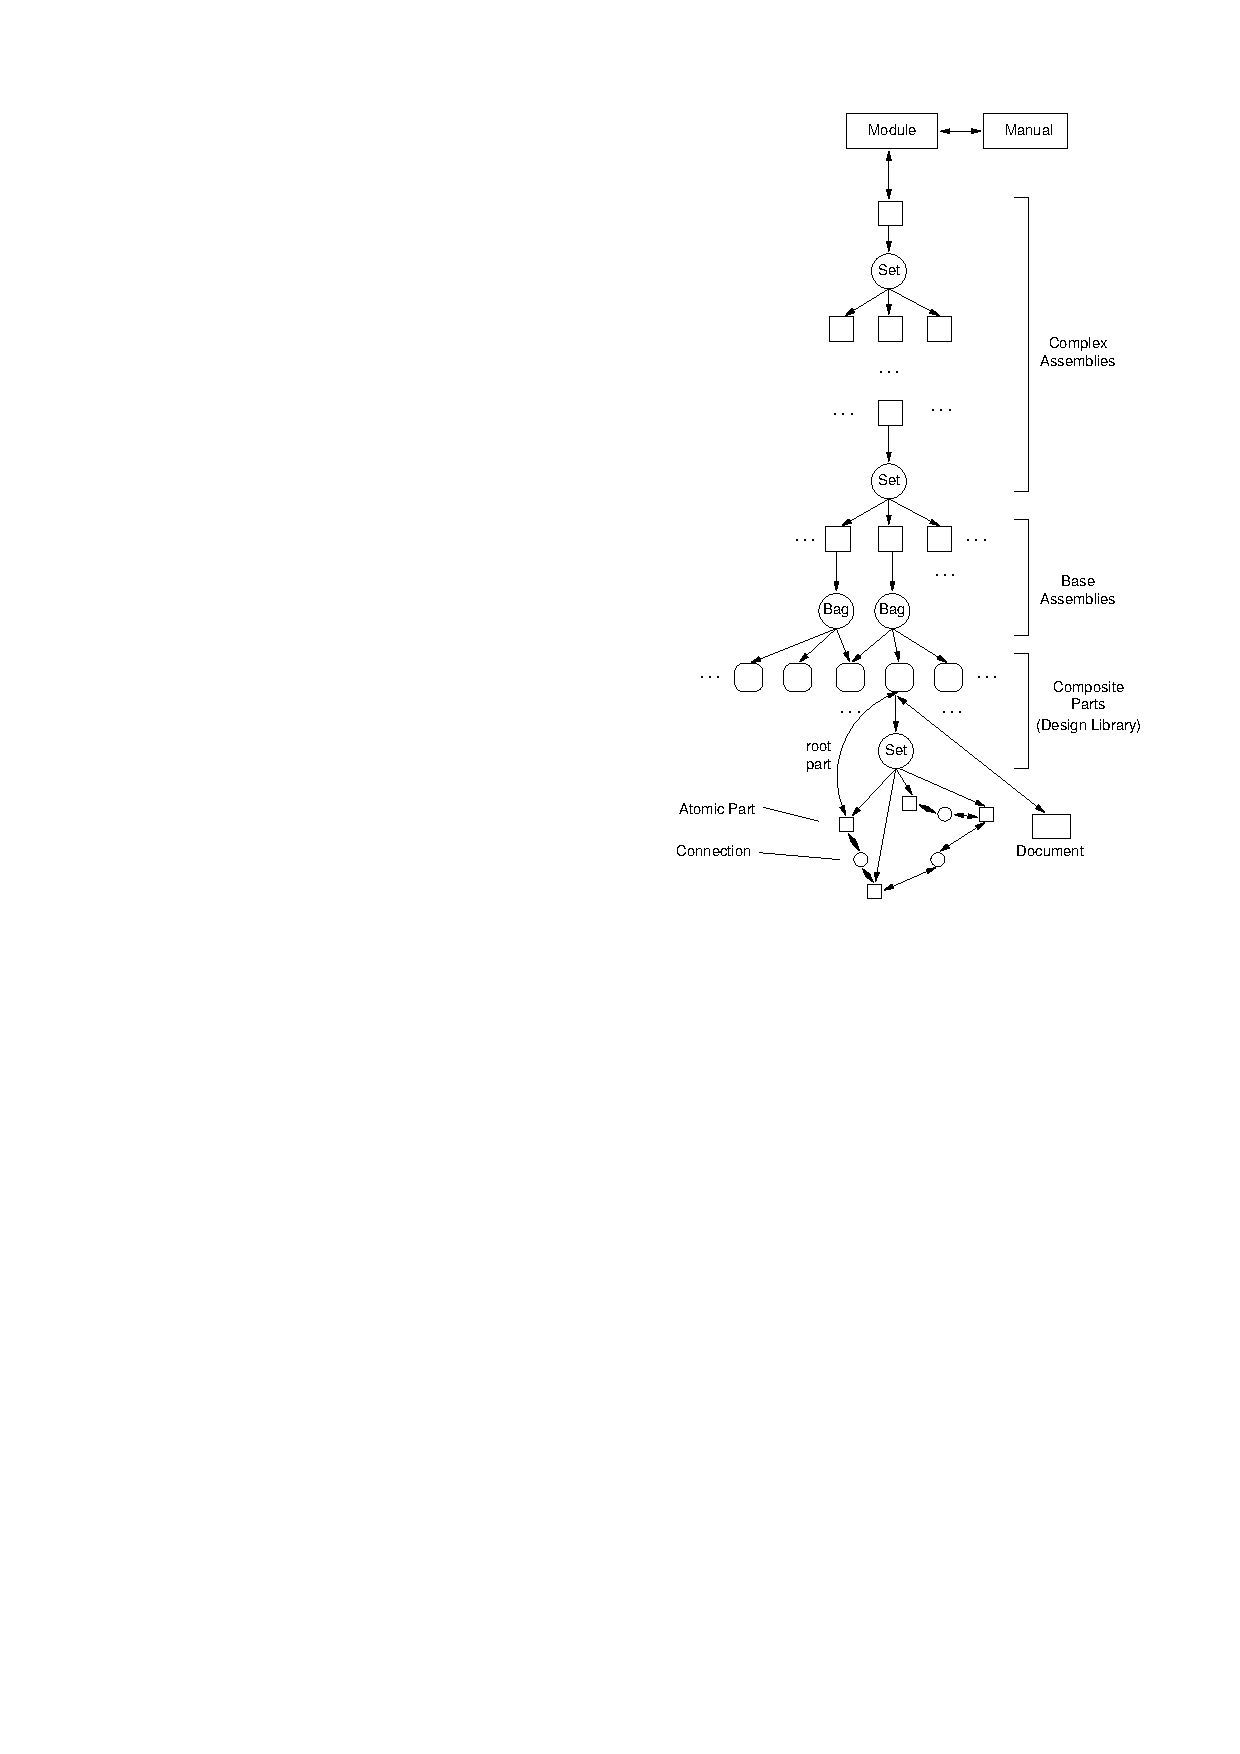
\includegraphics{stmbench7.pdf} \mycaption{The STMBench7
    data structure.}{This diagram is copied from the original
    STMBench7 paper~\cite{STMBench7}}.
  \label{fig:stmbench7}
\end{figure}

\paragraph{Backend data structures.} The benchmark data structures
are implemented using backend data structures. These backend data
structures must be implemented using each synchronisation
mechanism. To increase the fairness between synchronisation mechanisms
I kept these implementations as similar as possible. This guarantees
that any differences in performance are due to the synchronisation
mechanism and not to the backend data structure
implementation. Unfortunately the implementation used is rather
inefficient. In Section \ref{sec:impl:possible-extensions} I discuss
how this could be changed. It is worth drawing attention to two of the
backend data structures:

\begin{description}
\item[ID pool] An ID pool is a finite set of unique identifiers for a
  particular type of object. There is an ID pool for documents,
  composite parts, etc. When an object is created it gets an ID from
  the corresponding pool, if any are available. When an object is
  destroyed it returns the ID to the pool.
\item[Index] An index is a map of some key type to all the objects of
  a particular type. Most indexes have IDs taken from an ID pool as
  keys, but there is also an index of documents indexed by their
  titles and index of composite parts indexed by build date. When an
  object is created or destroyed it is added or removed, respectively,
  from the corresponding index or indices.
\end{description}

\subsection{Operations}
\label{sec:impl:operations}

STMBench7 supports four types of operations on its data structure,
which are summarised below. It is important to note that operations
can fail due to operation logic. This is not due to transactions aborting
or conflicting, but for example that ID pools are empty or that a
random traversal reached a base assembly with no composite parts. This
means that when looking at benchmark results it makes sense to look at
the total throughput and not only at the throughput of successful
operations.

\paragraph{Long traversals.} Long traversals traverse very large
numbers of objects. Most long traversals traverse the whole tree of
assemblies, and some also traverse the graph of atomic parts of all
composite parts. Most long traversals have a read-only and a
read-write variant. Long read-write traversals only perform write
operations on the attributes of atomic parts or documents --- they do
not modify structure.

\paragraph{Short traversals.} Short traversals reach much smaller
numbers of objects --- instead of traversing the whole tree of
assemblies, most short traversals take a random path from the root
assembly to a composite part or from an atomic part to the root
assembly. Most short traversals have read-only and read-write
variants, and the write operations are only on attributes of objects.

\paragraph{Short operations.} Short operations do not traverse the
data structure at all. Instead, they use the indexes to find all
objects of a type or find a random object. Again, most short
operations have read-only and read-write variants, and the write
operations are only on attributes of objects.

\paragraph{Structure modification operations.} Structure modifications
make major changes to the data structure. They add and remove
assemblies and composite parts and create and remove links between
them. This conflicts with all traversals, so the inclusion of
structure modifications in the benchmark workload severely impacts
performance, as shown in Section \ref{sec:impl:impact-struct-modif}.

\subsection{Design patterns}
\label{sec:impl:design-patterns}

The Java implementation of STMBench7 makes extensive use of object
oriented design patterns~\cite{GoF} to make it easy to extend the
benchmark with additional synchronisation approaches, such as
STMs. One of the challenges of porting the benchmark to Go was
understanding these patterns and how they can be adapted to a
non-object oriented language, and it was a good exercise of software
engineering skills. The most prominent patterns are described below.

\paragraph{Command.} Operation executors are an implementation of the
command pattern. Operation executors handle any top-level
synchronisation necessary before executing an operation. In the case
of the coarse grained locking approach this consists of acquiring the
global read-write lock, in a mode dependent of whether the operation
to be executed is read-only or read-write. The operation executor for
the medium grained locking approach is much more complex: a large
number of locks must be acquired in a specific order, according to
which operation is being executed. Writing this executor is rather
error prone, as the slightest mistake is likely to cause deadlock or
race conditions. The GVSTM operation executor, on the other hand,
simply wraps the operation to be executed in a call to the
\goFunc{Atomic} function.

\paragraph{Factory method and abstract factory.} STMBench7 provides
interfaces for all its benchmark and backend data structures, which are
used throughout the benchmark. Each synchronisation mechanism provides
its own implementations of these interfaces, along with the
corresponding factory methods and abstract factories. This layer of
abstraction makes it simple to, for example, change the implementation
of the backend data structures without touching the rest of the
codebase.

\paragraph{Builder.} Builders are used to create and destroy the
benchmark data structures while respecting the invariants of the
benchmark. They encapsulate the addition and removal of objects from
the corresponding indexes as well as the creation of other objects
associated with the object being created, such as the document of a
composite part and the children assemblies of a complex assembly.

\medskip

These patterns make the addition of new synchronisation approaches to
the benchmark simple: the new synchronisation approach must only
provide implementations of the data structures, an operation executor
and add its abstract factories to the main file. There is no need to
change any of the benchmark logic, such as its operations and
builders.

\subsection{Testing}
\label{sec:impl:testing}

As with any software engineering project, testing is important to
guarantee that my implementations of both the GVSTM and the benchmark
structures are correct. The original STMBench7 implementation included
both invariant tests on its data structures and opacity tests. Here I
explain my reasoning about what tests should be included in my
implementation.

\paragraph{Invariant tests.} The invariant tests of STMBench7 check
that both the benchmark and backend data structures are in a
consistent state. I implemented these tests as soon as I had
implemented the factories and builders of the data structures, which
proved to be useful: the tests helped me find a couple of bugs I had
overlooked, and allowed me to fix them before beginning to implement
the operations of the benchmark, which would have caused much more
complex errors. I kept running these tests as I implemented the
operations, which made it much more efficient for me to debug my code.

\paragraph{Opacity tests.} The opacity tests of STMBench7 check that
the execution of the benchmark by an STM satisfies the opacity
property described in Section \ref{sec:prep:techn-requ}. I did not
include the opacity tests in my implementation for three reasons:

\begin{description}
\item[Opacity is an STM property] \hfill \\
  The GVSTM algorithm is the same as that of the JVSTM, whose opacity
  property has already been shown. As such, the opacity tests would
  only tell me whether my implementation of the algorithm has bugs.
\item[Bugs are caught by invariant tests] \hfill \\
  Any bugs in the GVSTM implementation would cause large errors in any
  application using it. These errors would then cause the invariant
  tests to flag the error, so the opacity tests give me no new
  information.
\item[Heavy use of thread-local storage] \hfill \\
  As described in Section \ref{sec:impl:operations}, the short
  traversal operations make random traversals of the benchmark data
  structure. Opacity tests rely on retracing a concurrent execution
  serially, including the random parts. The Java implementation makes
  use of thread-local storage to keep per-thread reproducible random
  state in order to guarantee that the re-execution produces the same
  results. However, as discussed in Section
  \ref{sec:prep:thread-locals}, Go does not support thread-local
  storage, so a solution to this problem would be extremely complex,
  if at all possible.
\end{description}
In summary, the opacity tests would require a very substantial
engineering effort for no tangible benefit to this project, so I
decided not to implement them.

\subsection{Extensions}
\label{sec:impl:possible-extensions}

Here I discuss some extensions that could be made to my STMBench7
implementation. Most of them focus on making the benchmark results
more representative of real-world applications.

\paragraph{Implementing all 45 operations.} In my project proposal I
set out to only implement a subset of the original 45 operations of
STMBench7, and listed implementing all the operations as a possible
extension. In my project I achieved this extension goal. Although
implementing the benchmark as a whole was a much more ambitious goal
than I had expected, the addition of the remaining operations by
itself was reasonably simple thanks to the modular architecture of the
benchmark.

\paragraph{Efficient backend data structures.} As mentioned in Section
\ref{sec:impl:data-structures}, the implementations of the backend
data structures using locking approaches and STM are similar to
increase the fairness of the benchmark. The implementation in question
is very inefficient, because the data structure must be copied on
write to prevent concurrent access. A very valuable extension would be
to provide more efficient implementations of the backend data
structures. In the case of locking this would only involve removing
the copying operations. In the case of the GVSTM this would involve
the creation of complex versioned data structures such as sets and
maps. The JVSTM provides this as part of a library. The data
structures are based on persistent data
structures~\cite{PurelyFunctional}. The creation of such a library to
be distributed with the GVSTM would also make it much more appealing
to software engineers.

\paragraph{Containerising.} One of the strongest appeals of STMs is
that they scale much better than other approaches to large numbers of
cores. During my project I was only able to collect benchmark results
using my laptop, but it would be interesting to run the benchmark on
server class machines. To make this easier, it would be useful to
create an STMBench7 container to facilitate deployment on a cloud
computing platform.

\paragraph{Rewrite the benchmark to be fairer.} The method to create
and register a complex assembly is unfair to STMs: if the ID pool for
either complex or base assemblies is exhausted the method undoes all
its work. This involves a lot of operations on backend data
structures. Some STM implementations, such as the GVSTM extended with
abort and retry semantics (Section \ref{sec:impl:extensions}), could
simply abort or retry when they detect such an error, which would be
much more efficient.

\section{Repository overview}
\label{sec:impl:repository-overview}

One of my goals when proposing my project was to use it as a step
towards producing an open source library providing STM functionality
in Go. In order to evaluate my STM implementation, my project also had
to include the implementation of a benchmark for STMs. Because I
wanted this benchmark to be usable by other STM implementations, I
also needed to define an interface for STMs in Go. These three
``modules''~\cite[Section~1.1]{SoftwareArchitecture} of the project
should not necessarily be part of the same repository --- a software
engineer may only want to use the GVSTM, or only care about the
interface in order to produce their own STM implementation. For this
reason, the three modules should not necessarily be kept together in
the long run. In the scope of this project, however, it is much easier
to handle code submission and dependency management in a single
repository, so that is how I have structured my project. The
repository holding the source code of my project has one directory for
each of the modules. Their contents are summarised below.

\paragraph{STM interface.} The STM interface defined in this project
is reproduced fully in Listing \ref{lst:STMInterface}.

\paragraph{GVSTM.} The implementation of the GVSTM is reasonably short
--- less than 300 lines of code. That being said, the algorithm being
implemented is rather complex, especially in avoiding race conditions
in the garbage collection of old bodies. A good understanding of the
algorithm is necessary to understand the implementation of the
transaction objects and the active transaction records. The
implementation of versioned boxes and versioned bodies is reasonably
well contained.

\paragraph{STMBench7.} The STMBench7 benchmark is by far the largest
part of this project in terms of lines of code --- approximately
5000. The structure of the benchmark is described in Section
\ref{sec:impl:stmbench7}, and the organisation of source files is made
to resemble that of the Java implementation. Future versions of my
implementation may change this. Although I wrote all code submitted on
my own, my STMBench7 implementation is mostly a translation of the
Java version, with modifications to use the features of Go and the STM
interface I defined.

% \begin{figure}[h]
%   \centering 
\includegraphics{cuarms.pdf} \mycaption{Test
%   image.}{Kindly provided with the CL template.}
%   \label{fig:example}
% \end{figure}

% \begin{table}[h]
%   \centering
%   \begin{tabular}{| c | c |}
%     \hline
%     Float type & Working? \\
%     \hline
%     Figure & Check \\
%     Table & Check \\
%     Listing & Check \\
%     \hline
%   \end{tabular}
%   \mycaption{Test table.}{Shows whether the different types of
%   floats used are typeset as expected.}
%   \label{tbl:example}
% \end{table}


%%%%%%%%%%%%%%%%%%%%%%%%%%%%%%%%%%%%%%%%%%%%%%%
% Evaluation
%%%%%%%%%%%%%%%%%%%%%%%%%%%%%%%%%%%%%%%%%%%%%%%

\chapter{Evaluation}

In this chapter I recall the original goals of the project and
describe how they were achieved. I give quantitative results of
benchmarking the GVSTM with STMBench7 and qualitative conclusions from
using both locking approaches and the GVSTM to implement STMBench7. I
conclude with the real-world implications on the usability of the
GVSTM as an alternative to locking approaches in a variety of
scenarios.

\section{Success criteria}
\label{sec:eval:success-criteria}

\todo{Make sure to talk about testing.}

\section{Benchmark results}
\label{sec:eval:benchmark-results}

\todo{Talk bout engineering methodology, including
  \begin{itemize}
  \item Making sure ratio of failed operations is similar, so that
    results are not skewed.
  \item Benchmark run duration.
  \item Discarding outliers.
  \end{itemize}
}

\subsection{Metrics}
\label{sec:eval:metrics}

\paragraph{Total throughput.}

\paragraph{Maximum time to completion}

\paragraph{Time to completion histograms.}
May be interesting to show some histograms of TTC for some operation
types, but that may take up a lot of space. Could keep that in an
appendix.

\subsection{Impact of the number of threads}
\label{sec:eval:impact-numb-thre}

\subsection{Impact of structure modifications}
\label{sec:impl:impact-struct-modif}

Enabling structure modifications reduces throughput by more than one
order of magnitude for all synchronisation approaches.

\subsection{Workloads}
\label{sec:impl:workloads}

\paragraph{Read-only workload.}
\label{sec:impl:read-only-workload}

\paragraph{Read-dominated workload.}
\label{sec:eval:read-domin-workl}

\paragraph{Read-write workload.}
\label{sec:impl:read-write-workload}

\paragraph{Write-dominated workload.}
\label{sec:eval:write-domin-workl}


\subsection{Summary of results}
\label{sec:eval:summary-results}

Using the gvstm, long RW operations have very long TTCs, but read only
operations are not affected.

Using locking approaches, all operation types have similar TTCs. Can
relate this to different SLAs an application maintainer could have
with their users.

\section{Ease of use}
\label{sec:eval:ease-use}

\note{Due to the scope of this project, I couldn't do a usability
  study, so this is drawn from my own experience.}

\subsection{Implementing STMBench7}
\label{sec:eval:impl-stmb}

How easy it was to implement the executors:

\begin{itemize}
\item The GVSTM executor simply wraps the operation to execute in a
  call to Atomic.
\item The CG locking executor uses global read-write locks. When
  creating an executor for an operation, it determines whether it is
  read-only or read-write, and then acquires the appropriate lock
  before executing. Whether an operation is read-only or read-write is
  specified by the programmer, which has several problems:
  \begin{itemize}
  \item The approach does not allow the classification of arbitrary
    transactions that are not known at compile time. The GVSTM
    interface does not distinguish between RO and RW transactions and
    deals with that under the hood.
  \item Some transactions may perform some write operations in some
    executions but not others. Correct synchronisation would require
    these transactions to be classified as RW, which would make them
    perform worse than necessary when they happen to be RO.
  \item If someone misclassifies an operation as read-only, probably
    nothing fails in the program, but the results will be wrong
    because operations stop being atomic.
  \end{itemize}

\item The MG locking is much more complicated. It has read-write locks
  for each of several types of structures, as well as one read-write
  lock for each level of assemblies. I spent an afternoon fixing
  causes of deadlock and releases of not-acquired locks, even though I
  was pretty much only translating the algorithm. This shows how
  complicated programming with locks can be. (Part of the problem was
  that I forgot that the Java version uses reentrant locks, and Go
  does not have reentrant locks. I had to add some extra logic to make
  sure each lock is only acquired once.)
\end{itemize}

\subsection{Change of function signatures}
\label{sec:eval:change-funct-sign}

Any transactional function must receive a transaction object as an
argument. This means that it is difficult to use external libraries to
access shared memory transactionally, as the library would have to be
rewritten to pass around transaction objects.

A partial solution to this problem is the extension of making
transactional side effects using monads.

Locking would, to an extent, avoid this. That is, if only global locks
were used, the library need not know about any form of
synchronisation. However, as the implementation of the medium grained
locking approach has shown, an efficient locking approach will often
need more fine-grained control over locks, and locking state is passed
into the library.

\section{Real-world implications}
\label{sec:eval:real-world-impl}

Relate the results to real-world applications and SLAs that they may
have. The GVSTM offers extremely efficient read operations even in the
presence of writes, which locking approaches do not. It offers a
reasonably strong guarantee on the freshness of results of a read-only
transaction: if a read-only transaction begins after some other
transaction commits, the view of the read-only transactional will be
at least as fresh as the results of the committed transaction. This is
similar to linearisability.

%%%%%%%%%%%%%%%%%%%%%%%%%%%%%%%%%%%%%%%%%%%%%%%
% Conclusion
%%%%%%%%%%%%%%%%%%%%%%%%%%%%%%%%%%%%%%%%%%%%%%%

\chapter{Conclusion}

\section{Achievements}
\label{sec:conc:achievements}

\section{Lessons learnt}
\label{sec:conc:lessons-learnt}

Overall the project went well, and I do not regret any of the
technical decisions made. For students looking to do similar projects
in the future, I would recommend including some means of evaluating
more complex features, such as the extensions described in the
implementation chapter. If possible, make use of existing benchmarks
and add your own.

\section{Future work}
\label{sec:conc:future-work}

Summary of the extensions described in the implementation chapter.

%%%%%%%%%%%%%%%%%%%%%%%%%%%%%%%%%%%%%%%%%%%%%%%
% Bibliography
%%%%%%%%%%%%%%%%%%%%%%%%%%%%%%%%%%%%%%%%%%%%%%%
\addcontentsline{toc}{chapter}{Bibliography} \bibliography{biblio}

%%%%%%%%%%%%%%%%%%%%%%%%%%%%%%%%%%%%%%%%%%%%%%%
% Appendices
%%%%%%%%%%%%%%%%%%%%%%%%%%%%%%%%%%%%%%%%%%%%%%%

\appendix

\chapter{Project Proposal}
\label{cha:project-proposal}

\end{document}

%%% Local Variables:
%%% mode: latex
%%% TeX-master: t
%%% End:
